% =============================================================================
%  Dart-Throwing Robot — Codebase Technical Overview
%  CMU 16-745 Optimal Control & Reinforcement Learning
% =============================================================================
\documentclass[11pt,letterpaper]{article}

\usepackage[margin=1in]{geometry}
\usepackage{amsmath,amssymb,bm}
\usepackage{booktabs}
\usepackage{xcolor}
\usepackage{listings}
\usepackage{hyperref}
\usepackage{tikz}
\usepackage{pgfplots}
\pgfplotsset{compat=1.18}
\usepackage{enumitem}
\usepackage{fancyhdr}
\usepackage{titlesec}
\usepackage{mdframed}
\usepackage{graphicx}
\usepackage{array}
\usepackage{multirow}

% ---------- color palette ----------
\definecolor{cmu-red}{RGB}{196,18,48}
\definecolor{code-bg}{RGB}{245,245,245}
\definecolor{box-bg}{RGB}{235,243,255}
\definecolor{box-border}{RGB}{70,130,200}
\definecolor{warn-bg}{RGB}{255,248,235}
\definecolor{warn-border}{RGB}{200,140,40}
\definecolor{tip-bg}{RGB}{235,255,240}
\definecolor{tip-border}{RGB}{40,160,80}

% ---------- section styling ----------
\titleformat{\section}{\large\bfseries\color{cmu-red}}{{\thesection}}{0.8em}{}[\titlerule]
\titleformat{\subsection}{\normalsize\bfseries}{{\thesubsection}}{0.7em}{}
\titleformat{\subsubsection}{\normalsize\itshape}{}{0em}{}

% ---------- header / footer ----------
\pagestyle{fancy}
\fancyhf{}
\rhead{\textcolor{cmu-red}{\small CMU 16-745 — Dart Robot Codebase Overview}}
\lhead{\small \leftmark}
\cfoot{\thepage}

% ---------- code listing style ----------
\lstset{
  backgroundcolor=\color{code-bg},
  basicstyle=\ttfamily\small,
  breaklines=true,
  frame=single,
  rulecolor=\color{gray!40},
  keywordstyle=\color{blue}\bfseries,
  commentstyle=\color{gray!70},
  stringstyle=\color{orange!80!black},
  numbers=left,
  numberstyle=\tiny\color{gray},
  numbersep=6pt,
  language=Python,
  tabsize=4,
}

% ---------- callout boxes ----------
\newmdenv[
  backgroundcolor=box-bg,
  linecolor=box-border,
  linewidth=1.5pt,
  leftmargin=0pt, rightmargin=0pt,
  innerleftmargin=10pt, innerrightmargin=10pt,
  innertopmargin=8pt, innerbottommargin=8pt,
  skipabove=6pt, skipbelow=6pt,
]{infobox}

\newmdenv[
  backgroundcolor=warn-bg,
  linecolor=warn-border,
  linewidth=1.5pt,
  leftmargin=0pt, rightmargin=0pt,
  innerleftmargin=10pt, innerrightmargin=10pt,
  innertopmargin=8pt, innerbottommargin=8pt,
  skipabove=6pt, skipbelow=6pt,
]{warnbox}

\newmdenv[
  backgroundcolor=tip-bg,
  linecolor=tip-border,
  linewidth=1.5pt,
  leftmargin=0pt, rightmargin=0pt,
  innerleftmargin=10pt, innerrightmargin=10pt,
  innertopmargin=8pt, innerbottommargin=8pt,
  skipabove=6pt, skipbelow=6pt,
]{tipbox}

% ---------- math shortcuts ----------
\newcommand{\bq}{\bm{q}}
\newcommand{\bqdot}{\dot{\bm{q}}}
\newcommand{\bqdotdes}{\dot{\bm{q}}^*}
\newcommand{\bqdes}{\bm{q}^*}
\newcommand{\btau}{\bm{\tau}}
\newcommand{\R}[2]{\mathbf{R}_{#1}(#2)}
\newcommand{\norm}[1]{\left\lVert#1\right\rVert}

% =============================================================================
\begin{document}
% =============================================================================

% ---------- title page ----------
\begin{titlepage}
  \centering
  \vspace*{2cm}
  {\Huge\bfseries\color{cmu-red} Dart-Throwing Robot\\[0.4em]}
  {\Large Codebase Technical Overview\\[0.3em]}
  {\large CMU 16-745 — Optimal Control \& Reinforcement Learning\\[2cm]}

  \begin{infobox}
    \centering
    \textbf{What this document covers}\\[0.4em]
    \begin{tabular}{ll}
      \S1 & Project purpose and repository layout \\
      \S2 & Physical setup and coordinate system \\
      \S3 & Controller: cubic spline + PD torques + forward kinematics \\
      \S4 & Optimization: IK, overhand blend, knot optimizer \\
      \S5 & Flight integrator: RK45, drag model, event detection \\
      \S6 & Jacobian analysis and covariance propagation \\
      \S7 & End-to-end pipeline walkthrough \\
      \S8 & Debugging guide and common failure patterns \\
    \end{tabular}
  \end{infobox}

  \vfill
  {\small Last updated: May 2026}
\end{titlepage}

\tableofcontents
\newpage

% =============================================================================
\section{Project Purpose and Repository Layout}
% =============================================================================

\subsection{Goal}

The project builds a simulated 4-degree-of-freedom (4-DOF) robot arm that learns to throw darts accurately at a standard regulation dartboard. The three tracks of the course map directly to three phases of the problem:

\begin{center}
\begin{tabular}{>{\bfseries}l l l}
\toprule
Track & Problem & Key output \\
\midrule
A — Arm & Model the robot arm and plan joint trajectories & 12 spline knots \\
B — Ball & Model the dart's ballistic flight & Landing $(\Delta y, \Delta z)$ \\
C — Connect & Wire arm $\to$ flight $\to$ score; optimize end-to-end & Score, Monte Carlo \\
\bottomrule
\end{tabular}
\end{center}

\subsection{Repository Structure}

\begin{lstlisting}[language=bash, numbers=none]
src/dartrobot/              <- canonical source (import from here)
    constants.py            <- single source of truth for all numbers
    motion/
        controller.py       <- spline, PD, FK, MuJoCo simulation
        link_geometry.py    <- joint limits, inertias, clamp utility
    flight/
        forces.py           <- gravity + quadratic drag model
        integrator.py       <- RK45 flight ODE to board plane
        scoring.py          <- (Dy, Dz) -> dart score
    integration/
        ilqr_motion_targeting.py   <- IK + blend + retarget -> knots
        release_to_score.py        <- wiring: knots -> simulate -> score
        knot_landing_optimizer.py  <- scipy optimizer on knot vector
        jacobian_covariance.py     <- 2x6 Jacobian, covariance, MC
    rl/                     <- Stable-Baselines3 residual policy env
    spin/                   <- spin ablation study

*_SPEC/                     <- spec-test wrappers (import src/dartrobot)
run_debug_throw_pipeline_SPEC.py   <- MAIN DEBUGGING ENTRY POINT
run_sim.py                  <- simple physics sanity demo (no MuJoCo)
run_dart_robot_demo_SPEC.py <- full showcase pipeline
\end{lstlisting}

\begin{infobox}
  \textbf{Rule:} All real logic lives under \texttt{src/dartrobot/}. The \texttt{*\_SPEC/} directories are thin wrappers that run validation checks by importing from \texttt{src/dartrobot/}. Never edit the \texttt{\_SPEC} files to change behavior — edit the source modules instead.
\end{infobox}

% =============================================================================
\section{Physical Setup and Coordinate System}
% =============================================================================

\subsection{World Frame}

The coordinate system is fixed and right-handed:

\begin{center}
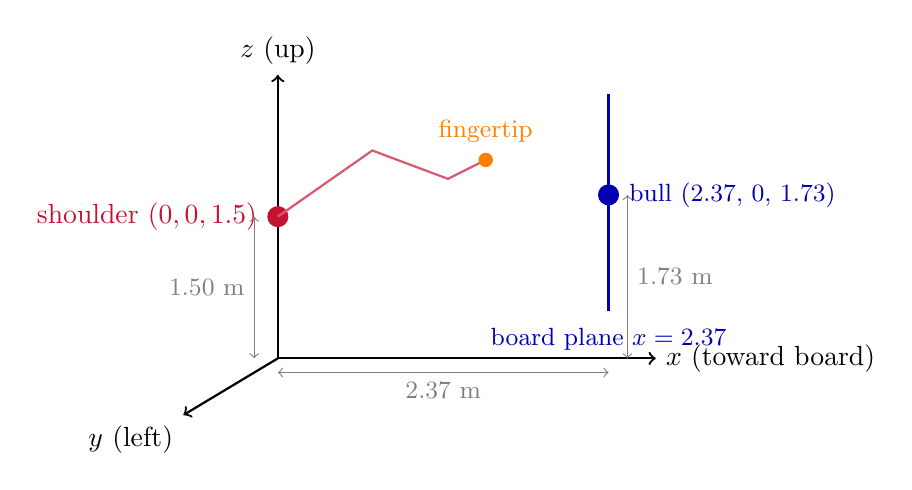
\begin{tikzpicture}[scale=1.2]
  % axes
  \draw[->, thick] (0,0) -- (4,0) node[right] {$x$ (toward board)};
  \draw[->, thick] (0,0) -- (0,3) node[above] {$z$ (up)};
  \draw[->, thick] (0,0) -- (-1,-0.6) node[below left] {$y$ (left)};

  % robot shoulder
  \filldraw[cmu-red] (0,1.5) circle (3pt) node[left=4pt] {shoulder $(0,0,1.5)$};

  % board
  \draw[thick, blue!70!black] (3.5,0.5) -- (3.5,2.8);
  \filldraw[blue!70!black] (3.5,1.73) circle (3pt)
    node[right=4pt, font=\small] {bull $(2.37,\,0,\,1.73)$};
  \node[blue!70!black, font=\small] at (3.5,0.2) {board plane $x=2.37$};

  % arm sketch
  \draw[thick, cmu-red!70] (0,1.5) -- (1.0,2.2) -- (1.8,1.9) -- (2.2,2.1);
  \filldraw[orange] (2.2,2.1) circle (2pt) node[above=3pt, font=\small] {fingertip};

  % distance annotation
  \draw[<->, gray] (0,-0.15) -- (3.5,-0.15) node[midway, below, font=\small] {2.37 m};
  \draw[<->, gray] (-0.25,0) -- (-0.25,1.5) node[midway, left, font=\small] {1.50 m};
  \draw[<->, gray] (3.7,0) -- (3.7,1.73) node[midway, right, font=\small] {1.73 m};
\end{tikzpicture}
\end{center}

\begin{warnbox}
  \textbf{Coordinate clarification:} The board is a \emph{vertical plane} at $x = 2.37$ m. Once the dart crosses this plane, we only care about \emph{where on the face} it landed. The face is parameterized by $(\Delta y,\, \Delta z)$ — offsets from the bullseye center $(y=0,\, z=1.73)$. The $x$-axis answers ``did the dart reach the board?''; the $y$- and $z$-axes answer ``where on the board?''
\end{warnbox}

\subsection{Physical Constants}

\begin{center}
\begin{tabular}{lll}
\toprule
Quantity & Value & Notes \\
\midrule
Shoulder mount & $(0,\,0,\,1.50)$ m & Fixed in world \\
Board plane & $x = 2.37$ m & Regulation oche distance \\
Bullseye height & $z = 1.73$ m & Center from floor \\
Upper arm & $L=0.30$ m, $m=2.1$ kg & \\
Forearm & $L=0.26$ m, $m=1.2$ kg & \\
Hand+dart & $L=0.08$ m, $m=0.4$ kg & Includes 22 g dart \\
MuJoCo timestep & 1 ms & \texttt{<option timestep="0.001">} \\
Throw duration & 0.2 s & Spline window \\
\bottomrule
\end{tabular}
\end{center}

\subsection{The 4-DOF Arm}

The arm has four joints. Joint angles are stored as the vector $\bq = [q_{\text{yaw}},\, q_{\text{sh}},\, q_{\text{el}},\, q_{\text{wr}}]$ in radians:

\begin{center}
\begin{tabular}{llll}
\toprule
Joint & Axis & Limits & Purpose \\
\midrule
Shoulder yaw & World $+z$ & $[-55°,\,+55°]$ & Left/right aim \\
Shoulder pitch & Local $y$ & $[-60°,\,+180°]$ & Arm elevation \\
Elbow & Local $y$ & $[-145°,\,0°]$ & Forearm fold \\
Wrist & Local $y$ & $[-70°,\,+70°]$ & Dart launch snap \\
\bottomrule
\end{tabular}
\end{center}

The cocked (starting) keyframe is $\bq_0 = [0°,\,-55°,\,-90°,\,-20°]$, which positions the arm raised above the bullseye height ready to throw overhand.

% =============================================================================
\section{Controller: Cubic Spline + PD Torques + Forward Kinematics}
% =============================================================================

\subsection{Trajectory Parameterization: Cubic Bezier Splines}

Rather than specifying torques directly, the controller follows a \emph{reference trajectory} computed from a small set of control points. For each joint $j$, a cubic Bezier curve is defined by four points:
\[
  P_0^{(j)} \;\text{(fixed start)},\quad
  P_1^{(j)},\; P_2^{(j)},\; P_3^{(j)} \;\text{(the 3 free knots)}
\]
The desired joint angle at normalized time $u = t/T \in [0,1]$ is:
\begin{equation}
  q_j^*(u) = (1-u)^3 P_0^{(j)}
           + 3(1-u)^2 u\, P_1^{(j)}
           + 3(1-u) u^2 P_2^{(j)}
           + u^3 P_3^{(j)}
  \label{eq:bezier}
\end{equation}
The desired joint velocity is obtained by differentiating Eq.~\eqref{eq:bezier} analytically with respect to $t$:
\begin{equation}
  \dot{q}_j^*(u) = \frac{1}{T}\left[
    -3(1-u)^2 P_0^{(j)}
    + 3(1-u)(1-3u) P_1^{(j)}
    + 3u(2-3u) P_2^{(j)}
    + 3u^2 P_3^{(j)}
  \right]
\end{equation}

With $T = 0.2$ s and 4 joints, the entire throw motion is encoded in exactly $4 \times 3 = 12$ numbers — the \textbf{policy vector} $\bm{\theta} \in \mathbb{R}^{12}$. Everything in the codebase that says \texttt{knots12} refers to this vector.

\begin{infobox}
  \textbf{Why Bezier?} Bezier curves are $C^\infty$ smooth, have analytic derivatives (no numerical differentiation), and the 3-knot-per-joint parameterization is compact enough for optimization while expressive enough to produce a dart-like whipping motion.
\end{infobox}

\subsection{Warm-Start: Minimum-Jerk Initialization}

Before any optimization, the knots are initialized using a \textbf{minimum-jerk trajectory}: the quintic polynomial that minimizes the integral of squared jerk $\int \dddot{q}^2 \, dt$:
\begin{equation}
  s(u) = 10u^3 - 15u^4 + 6u^5
\end{equation}
Given a start posture $\bq_0$ and a goal posture $\bq_{\text{goal}}$, the desired joint angle is $q_j(u) = q_{0,j} + s(u)\,(q_{\text{goal},j} - q_{0,j})$. The three Bezier knots are set by sampling this profile at $u = 1/3,\, 2/3,\, 1$. This gives a physically smooth initial trajectory that serves as the warm start for all optimization stages.

\subsection{PD Torque Controller}

At each 1 ms simulation timestep, the controller computes a torque command using a \textbf{Proportional-Derivative (PD)} law applied independently per joint:
\begin{equation}
  \btau = K_p \left(\bqdes - \bq\right) + K_d \left(\bqdotdes - \bqdot\right)
  \label{eq:pd}
\end{equation}

\begin{center}
\begin{tabular}{lll}
\toprule
Parameter & Value & Role \\
\midrule
$K_p$ (proportional gain) & 349 Nm/rad & Drives joint toward desired position \\
$K_d$ (derivative gain) & 1.89 Nm$\cdot$s/rad & Damps velocity error (prevents oscillation) \\
\bottomrule
\end{tabular}
\end{center}

An optional \textbf{feedforward term} adds a computed-torque component:
\begin{equation}
  \btau = \mathbf{M}\,\ddot{\bq}^* + K_p(\bqdes - \bq) + K_d(\bqdotdes - \bqdot)
\end{equation}
where $\mathbf{M} = \mathrm{diag}(1.2,\,1.0,\,0.8,\,0.3)$ kg$\cdot$m$^2$ is a diagonal inertia approximation and $\ddot{\bq}^*$ is the analytic Bezier acceleration. The feedforward term pre-commands the expected torque rather than waiting for an error to develop.

\textbf{Torque noise} (for Monte Carlo robustness studies) is added as:
\begin{equation}
  \btau_{\text{noisy}} = \btau + \underbrace{\sigma_{\text{add}}\,\bm{\epsilon}_1}_{\text{additive}} + \underbrace{\sigma_{\text{mult}}\,|\btau|\,\bm{\epsilon}_2}_{\text{multiplicative}},
  \quad \bm{\epsilon}_{1,2} \sim \mathcal{N}(\bm{0},\, \mathbf{I})
\end{equation}
with $\sigma_{\text{add}} = 0.5$ Nm and $\sigma_{\text{mult}} = 0.02$.

\subsection{Forward Kinematics (FK)}

FK answers: \emph{given joint angles $\bq$, where is the fingertip in world space?}

The arm uses a yaw-then-pitch chain. Each link segment $i$ has a unit direction vector:
\begin{equation}
  \hat{\bm{u}}_i = \mathbf{R}_z(q_{\text{yaw}})\, \mathbf{R}_y(Q_i)\, \hat{\bm{e}}_x
\end{equation}
where $Q_i$ is the \emph{cumulative} pitch angle:
\[
  Q_0 = q_{\text{sh}}, \quad Q_1 = q_{\text{sh}} + q_{\text{el}}, \quad Q_2 = q_{\text{sh}} + q_{\text{el}} + q_{\text{wr}}
\]
The fingertip (release site) world position is:
\begin{equation}
  \bm{p}_{\text{tip}} = \bm{o} + L_{\text{ua}}\,\hat{\bm{u}}_0 + L_{\text{fa}}\,\hat{\bm{u}}_1 + L_{\text{hand}}\,\hat{\bm{u}}_2
\end{equation}
where $\bm{o} = (0,0,1.5)$ m is the shoulder mount and the $L_i$ are the link lengths.

The fingertip \textbf{velocity} is obtained by differentiating with respect to $t$:
\begin{equation}
  \dot{\bm{p}}_{\text{tip}} = \sum_{i=0}^{2} L_i \left[
    \frac{\partial \hat{\bm{u}}_i}{\partial q_{\text{yaw}}}\dot{q}_{\text{yaw}} +
    \frac{\partial \hat{\bm{u}}_i}{\partial Q_i}\dot{Q}_i
  \right]
\end{equation}
At release time $t_r$, the 6D release state is:
\[
  \bm{s}_6 = [\bm{p}_{\text{tip}},\; \dot{\bm{p}}_{\text{tip}}] = [x_0, y_0, z_0, v_x, v_y, v_z]
\]
This is computed analytically in code (no numerical differentiation needed).

% =============================================================================
\section{Optimization: IK, Overhand Blend, and Knot Optimizer}
% =============================================================================

There are three distinct optimization layers, each solving a different sub-problem. They run sequentially, each feeding into the next.

\subsection{Layer 1 — Inverse Kinematics (Gauss–Newton)}

Given a 3D target position for the fingertip $\bm{p}_{\text{goal}}$, IK finds the joint angles $\bq$ that place the fingertip there. This is the reverse of FK, and it is iteratively solved using \textbf{Gauss–Newton}:

\begin{equation}
  \bq^{(k+1)} = \bq^{(k)} + \alpha\, \mathbf{J}^+\!\left(\bm{p}_{\text{goal}} - \bm{p}_{\text{tip}}(\bq^{(k)})\right)
  \label{eq:ik}
\end{equation}

\begin{center}
\begin{tabular}{lll}
\toprule
Symbol & Meaning & Value \\
\midrule
$\mathbf{J}$ & $3 \times 4$ Jacobian $\partial\bm{p}_{\text{tip}}/\partial\bq$ & analytic \\
$\mathbf{J}^+$ & Moore–Penrose pseudoinverse (handles non-square $J$) & \texttt{np.linalg.pinv}, rcond=$10^{-4}$ \\
$\alpha$ & Step size (prevents overshoot) & 0.38 \\
\multicolumn{2}{l}{Iterations} & 14 \\
\bottomrule
\end{tabular}
\end{center}

After IK, joint angles are clamped to their physical limits. The result $\bq_{\text{ik}}$ is the posture that puts the hand at the workspace goal — but it often produces a weak throw because it ignores the dynamics of the swing.

\subsection{Layer 2 — IK + Overhand Blend (the iLQR Stage)}

\subsubsection{The blending problem}
Pure IK gives accurate \emph{position} at release, but the resulting joint trajectory often has insufficient release speed. A hand-tuned ``overhand preset'' trajectory (stored as \texttt{DEFAULT\_MUJOCO\_OVERHAND\_THROW\_KNOTS\_SPEC}) is known to produce a strong throw $v_x \approx 6$--$8$ m/s. The strategy is to \textbf{blend} both:

\begin{equation}
  \bq_{\text{goal}} = (1 - \beta)\,\bq_{\text{overhand}} + \beta\,\bq_{\text{ik}}
  \label{eq:blend}
\end{equation}

The blend parameter $\beta \in [0, 1]$ controls the tradeoff:
\begin{itemize}[nosep]
  \item $\beta \to 1$: pure IK — good aim, possibly slow throw
  \item $\beta \to 0$: pure overhand preset — fast throw, poor aim
  \item $\beta = 0.42$ (default): 58\% speed from preset, 42\% aim correction from IK
\end{itemize}

\subsubsection{MuJoCo speed refinement loop}
After computing initial knots, the pipeline runs up to 6 MuJoCo simulations to check whether the release speed is acceptable:

\begin{lstlisting}
b = blend  # start at 0.42
for _ in range(6):
    sim = simulate_throw_mujoco(knots12, ...)
    if sim["release_state6"][3] >= 4.0:  # vx >= 4 m/s
        break
    b *= 0.88   # reduce IK influence, move toward overhand
    q_goal = (1-b)*q_overhand + b*q_ik
    knots12 = minimum_jerk_knots(q_start, q_goal)
\end{lstlisting}

\subsubsection{Landing retarget loop}
After knots are set, the pipeline runs a feedback correction loop: simulate the full throw, measure where it actually lands on the board $(\Delta y_{\text{actual}},\, \Delta z_{\text{actual}})$, compute the error, and nudge the workspace goal:

\begin{equation}
  \bm{p}_{\text{goal}}^{(k+1)} = \bm{p}_{\text{goal}}^{(k)} + \text{clip}\!\left(\begin{bmatrix}0 \\ 1.05\,e_y \\ 1.35\,e_z\end{bmatrix},\; \norm{\cdot} \leq 25\text{ mm}\right)
  \label{eq:retarget}
\end{equation}

where $e_y = \Delta y_{\text{target}} - \Delta y_{\text{actual}}$ and similarly for $e_z$. The 1.05/1.35 scale factors are heuristic gains accounting for the nonlinear mapping from hand position to board landing. The 25 mm cap prevents large errors from wildly moving the workspace goal. After each nudge: re-IK, re-blend, re-knots. Up to 6 iterations.

\begin{infobox}
  \textbf{Why ``iLQR'' in the name?} The function is named \texttt{solve\_ilqr\_motion\_knots\_for\_board\_deltas\_SPEC} as a placeholder for a proper iterative Linear Quadratic Regulator. The current implementation uses the IK+blend heuristic described above rather than a true iLQR trajectory optimizer. This is a known open item.
\end{infobox}

\subsection{Layer 3 — Knot Optimizer (Nelder-Mead, Stage S4)}

After the iLQR stage (S3) produces initial knots, an optional \textbf{derivative-free optimizer} refines the full 12D knot vector to minimize a scalar loss:

\begin{equation}
  \mathcal{L}(\bm{\theta}) =
    \underbrace{e_y^2 + e_z^2}_{\text{L2 to target}}
    + \underbrace{\lambda_1 \cdot \mathbf{1}[\text{no plane hit}]}_{\text{plane-miss penalty}}
    + \underbrace{\lambda_2 \cdot \left(\frac{r - r_{\max}}{1000}\right)^2 \mathbf{1}[r > r_{\max}]}_{\text{off-face penalty}}
  \label{eq:knot-loss}
\end{equation}

with $\lambda_1 = 50{,}000$, $\lambda_2 = 120$, $r_{\max} = 170$ mm. The penalties strongly guide the optimizer to keep throws on the board face before worrying about L2 accuracy.

\textbf{Nelder-Mead} is used because:
\begin{enumerate}[nosep]
  \item The inner function (MuJoCo simulation) is not differentiable — gradients are unavailable
  \item Nelder-Mead is a simplex method that requires only function evaluations
  \item It maintains $n+1 = 13$ candidate solutions in the 12D space, iteratively replacing the worst with a reflected/contracted/expanded vertex
\end{enumerate}

\textbf{Multi-restart}: the optimizer runs $N$ times from different random perturbations of the initial knots ($\sigma = 0.12$ rad per knot), keeping the best result. This helps escape local minima in the non-convex loss landscape.

% =============================================================================
\section{Flight Integrator: RK45, Drag Model, and Event Detection}
% =============================================================================

\subsection{Force Model: Point Mass with Quadratic Drag}

Once released, the dart is treated as a \textbf{point mass} subject to two forces. The state is $\bm{s} = [x,\, y,\, z,\, v_x,\, v_y,\, v_z]^\top \in \mathbb{R}^6$.

\textbf{Gravity:}
\begin{equation}
  \bm{F}_g = [0,\; 0,\; -mg]^\top, \quad m = 0.022\text{ kg},\quad g = 9.81\text{ m/s}^2
\end{equation}

\textbf{Quadratic aerodynamic drag:}
\begin{equation}
  \bm{F}_d = -\frac{1}{2}\rho\, C_d\, A\, \norm{\bm{v}_{\text{rel}}}\,\bm{v}_{\text{rel}},
  \quad \bm{v}_{\text{rel}} = \bm{v} - \bm{v}_{\text{wind}}
  \label{eq:drag}
\end{equation}

\begin{center}
\begin{tabular}{lll}
\toprule
Parameter & Symbol & Value \\
\midrule
Air density & $\rho$ & 1.225 kg/m$^3$ \\
Drag coefficient & $C_d$ & 0.47 (sphere approximation) \\
Cross-section area & $A$ & $3.0 \times 10^{-4}$ m$^2$ ($\approx20$ mm barrel) \\
\bottomrule
\end{tabular}
\end{center}

\begin{warnbox}
  \textbf{Drag magnitude:} At $v = 6$ m/s with no wind, drag is approximately $1.5\%$ of gravitational acceleration — small but non-negligible over 2.37 m. At 7 m/s, drag deflects the landing by $\approx2$--$3$ mm relative to no-drag, which matters at dart precision scales.
\end{warnbox}

The full ODE right-hand side is:
\begin{equation}
  \frac{d\bm{s}}{dt} = f(\bm{s}) =
  \begin{bmatrix}
    v_x,\; v_y,\; v_z,\;
    a_x(\bm{v}),\; a_y(\bm{v}),\; a_z(\bm{v})
  \end{bmatrix}^\top
\end{equation}

\subsection{Integration Method: RK45 with Adaptive Stepping}

The flight ODE is integrated using \textbf{scipy's \texttt{solve\_ivp}} with the \textbf{RK45} method (Dormand-Prince). RK45 is a \emph{Runge-Kutta} scheme that evaluates the derivative $f(\bm{s})$ at 6 intermediate points within each step, combining them with optimized weights to achieve 4th-order accuracy while also computing a 5th-order estimate for error control.

\textbf{Adaptive step size:} At each proposed step of size $h$, the method computes both a 4th-order estimate $\hat{\bm{s}}_{k+1}^{(4)}$ and a 5th-order estimate $\hat{\bm{s}}_{k+1}^{(5)}$. The difference $\bm{\delta} = \hat{\bm{s}}^{(5)} - \hat{\bm{s}}^{(4)}$ approximates the local truncation error. The step is accepted if:
\begin{equation}
  \max_i \frac{|\delta_i|}{\texttt{atol} + \texttt{rtol}\cdot|s_i|} \leq 1
\end{equation}
and rejected (halving $h$) otherwise. The tolerances used are $\texttt{rtol} = 10^{-8}$, $\texttt{atol} = 10^{-10}$, giving sub-micrometer precision on the landing coordinates.

\subsection{Terminal Event Detection: Board Plane Crossing}

Rather than integrating to a fixed end time and then interpolating, \texttt{solve\_ivp} supports \textbf{event detection}: a condition function is registered that fires when $x(t) - 2.37 = 0$. The event is configured with:
\begin{itemize}[nosep]
  \item \texttt{terminal = True} — stop integration immediately when event fires
  \item \texttt{direction = +1} — only trigger on \emph{forward} crossings ($v_x > 0$)
\end{itemize}

scipy uses the \textbf{dense output} (a continuous polynomial interpolant computed alongside the RK45 steps) to find the exact zero-crossing time $t^*$ via bisection, without needing to take smaller steps. At $t^*$:
\begin{equation}
  \Delta y = y(t^*), \quad \Delta z = z(t^*) - 1.73
\end{equation}

If no forward crossing is detected within \texttt{max\_time\_s = 3.0 s}, the function returns a ``miss'' sentinel (\texttt{hit = False}).

% =============================================================================
\section{Jacobian Analysis and Covariance Propagation}
% =============================================================================

\subsection{The 2×6 Landing Jacobian}

The Jacobian quantifies how small changes in the 6D release state $\bm{s}_6$ translate to changes in the 2D board landing $\bm{\ell} = [\Delta y,\, \Delta z]^\top$:

\begin{equation}
  \mathbf{J} = \frac{\partial \bm{\ell}}{\partial \bm{s}_6} \in \mathbb{R}^{2 \times 6}
\end{equation}

Because the flight integrator has no closed-form derivative, $\mathbf{J}$ is computed via \textbf{forward finite differences}:
\begin{equation}
  J_{ij} = \frac{\ell_i(\bm{s}_6 + \varepsilon\,\bm{e}_j) - \ell_i(\bm{s}_6)}{\varepsilon}, \quad \varepsilon = 10^{-4}
\end{equation}
This requires 6 additional flight integrations beyond the nominal (one per release state component). The resulting Jacobian has rows $[\partial\Delta y,\, \partial\Delta z]$ and columns $[\partial x_0,\, \partial y_0,\, \partial z_0,\, \partial v_x,\, \partial v_y,\, \partial v_z]$.

\subsection{First-Order Covariance Propagation}

If the release state has Gaussian uncertainty $\bm{s}_6 \sim \mathcal{N}(\bar{\bm{s}}_6,\, \boldsymbol{\Sigma}_{\text{release}})$, the landing uncertainty is approximated (to first order) as:
\begin{equation}
  \boldsymbol{\Sigma}_{\text{land}} \approx \mathbf{J}\,\boldsymbol{\Sigma}_{\text{release}}\,\mathbf{J}^\top \in \mathbb{R}^{2 \times 2}
  \label{eq:cov-prop}
\end{equation}

This is much faster than Monte Carlo (6 integrations vs.\ hundreds) and gives an ellipse in the $(\Delta y, \Delta z)$ plane that can be visualized alongside MC scatter.

\subsection{Sensitivity Ranking}

To understand which release variable matters most, the covariance is decomposed per-component:
\begin{equation}
  \boldsymbol{\Sigma}_{\text{land},\,i} = \mathbf{J}\,\tilde{\boldsymbol{\Sigma}}_i\,\mathbf{J}^\top,
  \quad \tilde{\boldsymbol{\Sigma}}_i = \text{diag}(0,\ldots,\sigma_{ii}^2,\ldots,0)
\end{equation}
The trace $\text{tr}(\boldsymbol{\Sigma}_{\text{land},\,i})$ gives the total landing variance attributable to uncertainty in release component $i$ alone. This tells you — \emph{is it more important to control the release velocity in $x$, or the release height $z$?}

% =============================================================================
\section{End-to-End Pipeline Walkthrough}
% =============================================================================

The complete chain from a board target to a dart score is:

\begin{center}
\begin{tikzpicture}[
  node distance=0.9cm,
  box/.style={rectangle, draw=box-border, fill=box-bg, rounded corners, minimum width=9cm, minimum height=0.65cm, font=\small, align=left},
  label/.style={font=\scriptsize\ttfamily, text=gray},
  arrow/.style={->, thick, color=cmu-red!70}
]
  \node[box] (target) {\textbf{Input:} Board target $(\Delta y_\text{goal},\, \Delta z_\text{goal})$ in meters from bullseye};
  \node[box, below=of target] (ws) {\textbf{Workspace goal:} map $(\Delta y, \Delta z)$ $\to$ 3D hand position $\bm{p}_\text{goal}$};
  \node[box, below=of ws] (ik) {\textbf{IK (Gauss–Newton, 14 iter):} $\bm{p}_\text{goal} \to \bq_\text{ik}$};
  \node[box, below=of ik] (blend) {\textbf{Blend ($\beta=0.42$):} $\bq_\text{goal} = (1-\beta)\bq_\text{overhand} + \beta\bq_\text{ik}$};
  \node[box, below=of blend] (minjerk) {\textbf{Minimum-jerk knots:} $\bq_0 \to \bq_\text{goal}$ $\Rightarrow$ \texttt{knots12} (S1)};
  \node[box, below=of minjerk] (refine) {\textbf{MuJoCo speed check ($\leq 6$ iter):} reduce $\beta$ if $v_x < 4$ m/s (S2)};
  \node[box, below=of refine] (retarget) {\textbf{Landing retarget ($\leq 6$ iter):} nudge $\bm{p}_\text{goal}$ from board error, re-IK (S3)};
  \node[box, below=of retarget] (optknots) {\textbf{Knot optimizer (Nelder-Mead, $N$ restarts):} minimize $\mathcal{L}(\bm{\theta})$ (S4)};
  \node[box, below=of optknots] (mujoco) {\textbf{MuJoCo simulation:} \texttt{knots12} $\to$ PD torques $\to$ \texttt{release\_state6}};
  \node[box, below=of mujoco] (flight) {\textbf{RK45 flight:} \texttt{release\_state6} $\to$ board crossing at $x=2.37$};
  \node[box, below=of flight] (score) {\textbf{Output:} $(\Delta y_\text{actual},\, \Delta z_\text{actual})$ $\to$ dart score (BULL / T20 / etc.)};

  \draw[arrow] (target) -- (ws);
  \draw[arrow] (ws) -- (ik);
  \draw[arrow] (ik) -- (blend);
  \draw[arrow] (blend) -- (minjerk);
  \draw[arrow] (minjerk) -- (refine);
  \draw[arrow] (refine) -- (retarget);
  \draw[arrow] (retarget) -- (optknots);
  \draw[arrow] (optknots) -- (mujoco);
  \draw[arrow] (mujoco) -- (flight);
  \draw[arrow] (flight) -- (score);

  % stage labels
  \node[label, right=0.3cm of minjerk] {iLQR stage};
  \node[label, right=0.3cm of retarget] {iLQR stage};
  \node[label, right=0.3cm of optknots] {knot optimizer};
\end{tikzpicture}
\end{center}

\subsection{Key Data Types at Each Stage}

\begin{center}
\begin{tabular}{lll}
\toprule
Stage output & Type & Meaning \\
\midrule
$\bm{p}_{\text{goal}}$ & $\mathbb{R}^3$ & 3D target for fingertip in world frame \\
$\bq_{\text{ik}}$, $\bq_{\text{goal}}$ & $\mathbb{R}^4$ & Joint angle postures (rad) \\
\texttt{knots12} & $\mathbb{R}^{12}$ & Bezier control points, 3 per joint \\
\texttt{release\_state6} & $\mathbb{R}^6$ & $[x,y,z,v_x,v_y,v_z]$ at fingertip \\
$(\Delta y, \Delta z)$ & $\mathbb{R}^2$ & Landing offset from bullseye (m) \\
score & int & Dart score: 0 (miss) to 60 (T20) \\
\bottomrule
\end{tabular}
\end{center}

% =============================================================================
\section{Debugging Guide and Common Failure Patterns}
% =============================================================================

\subsection{Primary Debugging Tool}

The primary debugging entry point is:
\begin{lstlisting}[language=bash, numbers=none]
python run_debug_throw_pipeline_SPEC.py \
    --preset-set s20 \
    --maxiter 80 \
    --n-restarts 10
\end{lstlisting}
This runs all 4 stages (S1--S4) for each target preset and prints a table:
\begin{center}
\texttt{preset\ \ \ \ \ stage\ \ \ \ \ r\_mm\ \ \ ey\_mm\ \ ez\_mm\ \ vx\ \ vz\ \ |v|\ \ face}
\end{center}
\begin{itemize}[nosep]
  \item \textbf{r\_mm} — radial distance of landing from target (0 = perfect)
  \item \textbf{ey\_mm / ez\_mm} — signed error in Y and Z directions (mm)
  \item \textbf{face} — \texttt{Y}/\texttt{N} whether the dart hit the dartboard disk ($r \leq 170$ mm)
  \item \textbf{vx, |v|} — release velocity components (m/s)
\end{itemize}

\subsection{Common Failure Patterns}

\begin{center}
\renewcommand{\arraystretch}{1.4}
\begin{tabular}{>{\bfseries}p{3.5cm} p{5.5cm} p{5cm}}
\toprule
Symptom & Likely cause & Where to look \\
\midrule
$v_x < 4$ m/s at release &
  IK blend pulling arm to a slow posture; speed refinement loop didn't converge &
  \texttt{refine\_min\_release\_vx\_mps}, \texttt{refine\_max\_iters} in \texttt{ilqr\_motion\_targeting.py:74} \\
\addlinespace
Consistent negative \texttt{ez\_mm} &
  Landing persistently below aim: release height too low, pitch too shallow, or release time too late relative to spline peak &
  \texttt{KEYFRAME\_SHOULDER\_DEG}, \texttt{DEFAULT\_MUJOCO\_OVERHAND\_RELEASE\_TIME\_S\_SPEC} in \texttt{controller.py:412} \\
\addlinespace
\texttt{face = N} for all targets &
  Dart crosses $x=2.37$ far off the disk; often a yaw problem or the arm is swinging sideways &
  \texttt{KEYFRAME\_SHOULDER\_YAW\_DEG}, shoulder yaw knots in the overhand preset \\
\addlinespace
S2 worse than S1 &
  MuJoCo $v_x$ refine is over-reducing $\beta$, pulling the blend too far toward the overhand preset and destroying aim &
  \texttt{blend\_ik\_with\_overhand} default value, \texttt{refine\_max\_iters} \\
\addlinespace
S4 small \texttt{opt\_fun} but large \texttt{r\_mm} &
  Nelder-Mead converged to a local minimum; the loss landscape has poor conditioning near the off-face penalty boundary &
  Increase \texttt{--n-restarts}, reduce \texttt{restart\_sigma\_rad}, check \texttt{plane\_miss\_penalty} magnitude \\
\addlinespace
Retarget loop diverges &
  25 mm workspace step cap is too small relative to the board error; needs more iterations or a coarser first pass &
  \texttt{\_LANDING\_RETARGET\_MAX\_WS\_STEP\_M} in \texttt{ilqr\_motion\_targeting.py:32} \\
\bottomrule
\end{tabular}
\end{center}

\subsection{Module-Level Debugging Checklist}

\begin{enumerate}
  \item \textbf{FK sanity:} call \texttt{release\_site\_fk\_SPEC(q\_start4)} and verify the fingertip is near $(0.6,\, 0,\, 1.75)$ m — arm raised, about 0.6 m in front of the shoulder mount.
  \item \textbf{Flight sanity:} call \texttt{integrate\_until\_board\_SPEC([0,0,1.73, 7,0,2])} — should return \texttt{hit=True} with $\Delta y \approx 0$, $\Delta z \approx +0.1$ m (the dart arcs upward slightly then falls to 1.73 m by the board).
  \item \textbf{Release velocity direction:} check that \texttt{release\_state6[3]} ($v_x$) is positive and $>4$ m/s. Negative $v_x$ means the arm is swinging backward at release.
  \item \textbf{Jacobian sign check:} \texttt{jacobian\_landing\_wrt\_release\_SPEC} column 3 ($\partial\Delta z/\partial v_z$) should be positive — releasing upward should make the dart land higher.
  \item \textbf{Scoring geometry:} \texttt{score\_from\_deltas\_SPEC(0, 0)} should return 50 (inner bull).
\end{enumerate}

% =============================================================================
\section*{Appendix: Key Constants Quick Reference}
% =============================================================================
\addcontentsline{toc}{section}{Appendix: Key Constants Quick Reference}

All constants are defined in \texttt{src/dartrobot/constants.py}. Never hard-code these values in other files.

\begin{center}
\begin{tabular}{lll}
\toprule
Constant name & Value & Physical meaning \\
\midrule
\texttt{OCHE\_TO\_BOARD\_X\_M} & 2.37 m & Board plane location \\
\texttt{BULLSEYE\_CENTER\_Z\_M} & 1.73 m & Bull height from floor \\
\texttt{SHOULDER\_MOUNT\_Z\_M} & 1.50 m & Robot arm attachment height \\
\texttt{THROW\_DURATION\_S} & 0.2 s & Spline time window \\
\texttt{N\_POLICY\_PARAMETERS} & 12 & 4 joints $\times$ 3 knots \\
\texttt{RELEASE\_TIME\_SIGMA\_S} & 0.01 s & Jitter in release timing \\
\texttt{DEFAULT\_MUJOCO\_OVERHAND\_PD\_KP\_SPEC} & 349 Nm/rad & Proportional gain \\
\texttt{DEFAULT\_MUJOCO\_OVERHAND\_PD\_KD\_SPEC} & 1.89 Nm$\cdot$s/rad & Derivative gain \\
\texttt{DEFAULT\_MUJOCO\_OVERHAND\_RELEASE\_TIME\_S\_SPEC} & 0.10 s & Nominal release time \\
\texttt{R\_BOARD\_MISS\_MM} & 170 mm & Outer edge of scoring area \\
\bottomrule
\end{tabular}
\end{center}

% =============================================================================
\end{document}
% =============================================================================
